\documentclass{beamer}

\usetheme{Madrid}

% Pachete
\usepackage[utf8]{inputenc}
\usepackage{graphicx}
\usepackage{xcolor}
\usepackage{tikz}
\usetikzlibrary{shapes,arrows}

% DEFINIRE CULOARE MOV
\definecolor{myPurple}{RGB}{128,0,128}

% Aplicare culoare peste tot
\setbeamercolor{structure}{fg=myPurple}
\setbeamercolor{frametitle}{bg=myPurple, fg=white}
\setbeamercolor{title}{fg=white}
\setbeamercolor{block title}{bg=myPurple, fg=white}

% Elimină iconițe inutile
\setbeamertemplate{navigation symbols}{}

% Info
\title{Face Recognition}
\author{Damian Alexandru \\ Horneț Alex-Andrei}
\institute{Faculty of Mathematics and Computer Science \\ University of Bucharest \\ IAVA}
\date{}


\begin{document}

% 1
\begin{frame}
    \titlepage
\end{frame}

% 2
\begin{frame}{Mid Term Presentation}
    \tableofcontents
\end{frame}

\section{Problem Definition}

% 3
\begin{frame}{Problem Definition}
\begin{itemize}
    \item Building a face recognition system that identifies a person from a given image
    \item Input: random image of someone
    \item Output: the name of the person
    \item Challenges: bad lighting, modified angles, blurring
\end{itemize}
\end{frame}

% 4
\begin{frame}{Problem Definition}
\begin{itemize}
    \item Usage: security, authentication
    \item Problem type: classification 
    \item Computer vision component
\end{itemize}
\end{frame}

\section{Datasets}

% 5
\begin{frame}{Dataset - CelebA}
\begin{itemize}
    \item 200,000 face images of 10,000 identities
    \item Well-aligned and higher quality images
    \item Each image has 40 attribute labels (sex, glasses, smile, etc.)
\end{itemize}
\end{frame}

% 6
\begin{frame}{Dataset - Motivation}
\begin{itemize}
    \item Large dataset: good for training models
    \item Rich annotations (attributes)
    \item More consistent image quality
\end{itemize}
\end{frame}

\section{State of the Art}

\begin{frame}{Proposed Model Pipeline}
\centering
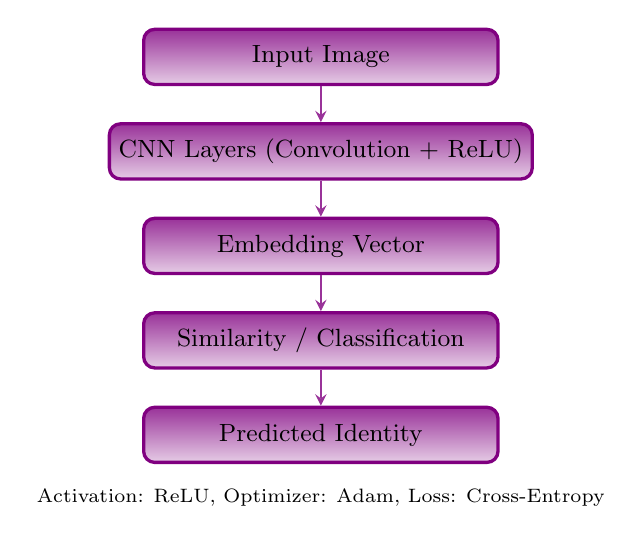
\begin{tikzpicture}
\tikzset{
    gradient block/.style={
        rectangle, 
        minimum width=4.5cm, minimum height=0.7cm, 
        text centered, rounded corners,
        top color=myPurple!80, bottom color=myPurple!20, 
        draw=myPurple, very thick,
        font=\small
    },
    arrow/.style={
        thick, ->, >=stealth, draw=myPurple!80
    }
}
% Noduri cu coordonate absolute
\node[gradient block] (input)   at (0,  0)    {Input Image};
\node[gradient block] (cnn)     at (0, -1.2)  {CNN Layers (Convolution + ReLU)};
\node[gradient block] (emb)     at (0, -2.4)  {Embedding Vector};
\node[gradient block] (compare) at (0, -3.6)  {Similarity / Classification};
\node[gradient block] (output)  at (0, -4.8)  {Predicted Identity};

% Sageti
\draw[arrow] (input)   -- (cnn);
\draw[arrow] (cnn)     -- (emb);
\draw[arrow] (emb)     -- (compare);
\draw[arrow] (compare) -- (output);

% Nota de jos
\node[font=\scriptsize] at (0, -5.6) {Activation: ReLU, Optimizer: Adam, Loss: Cross-Entropy};
\end{tikzpicture}
\end{frame}
% 8
\begin{frame}{State of the Art - Model Setup}
\begin{itemize}
    \item Model type: simple CNN for embeddings
    \item Activation functions: ReLU in hidden layers, Softmax for output
    \item Optimizer: Adam (adaptive learning rate)
\end{itemize}
\end{frame}

% 9
\begin{frame}{State of the Art - Training Details}
\begin{itemize}
    \item Loss function: Cross-entropy (for classification)
    \item Training setup: batch size of 32 and 20 epochs
    \item Reasoning: simple configuration, easy to implement and test
\end{itemize}
\end{frame}

\section{Conclusion}

% 10
\begin{frame}{Conclusion}
\begin{itemize}
    \item Proposed a simple CNN model with ReLU, Softmax, Adam, and Cross-Entropy
    \item Selected a dataset suitable for our project (CelebA)
    \item Next steps: implement the model, train on dataset, evaluate performance
\end{itemize}
\end{frame}

\end{document}